\documentclass[tikz,border=10pt]{standalone}
\usepackage{tikz}
\usetikzlibrary{shapes.geometric, arrows.meta}

% Define styles for nodes and arrows
\tikzstyle{startstop} = [rectangle, rounded corners, minimum width=3cm, minimum height=1cm,text centered, draw=black, fill=red!30]
\tikzstyle{process} = [rectangle, minimum width=3cm, minimum height=1cm, text centered, draw=black, fill=orange!30]
\tikzstyle{decision} = [diamond, minimum width=3cm, minimum height=1cm, text centered, draw=black, fill=green!30]
\tikzstyle{arrow} = [thick,->,>=stealth]

\begin{document}
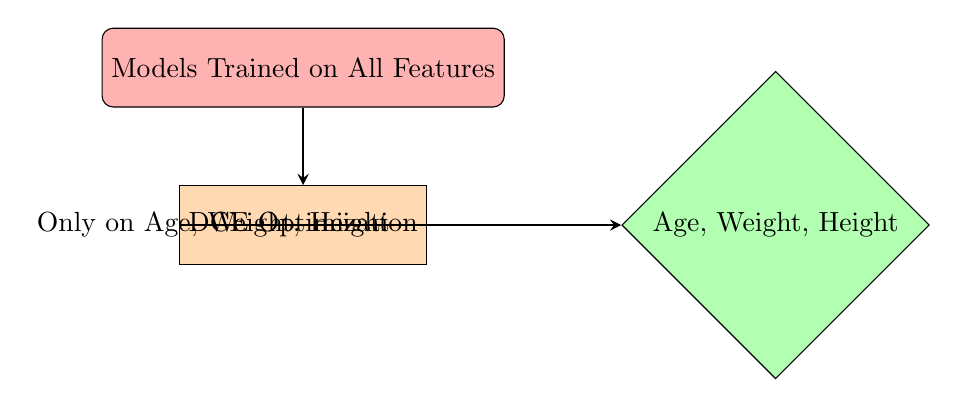
\begin{tikzpicture}[node distance=2cm]

    % Nodes
    \node (models) [startstop] {Models Trained on All Features};
    \node (dce_optimization) [process, below of=models] {DCE Optimization};
    \node (age_weight_height) [decision, right of=dce_optimization, xshift=4cm] {Age, Weight, Height};

    % Arrows
    \draw [arrow] (models) -- (dce_optimization);
    \draw [arrow] (dce_optimization.west) -- node[anchor=east] {Only on Age, Weight, Height} (age_weight_height);

\end{tikzpicture}
\end{document}